\chapter{力、相空間與守恆定律}

\lectureoverview{運動定律不能只把熟悉的物理量彼此聯繫起來。它還必須指定系統的狀態，描述該狀態如何從一個時刻演變到下一個時刻，並揭示運動過程中哪些區別與物理量得以保留。我們將先檢驗一條看似合理、實則錯誤的力定律，再將狀態從位置擴展到相空間，最後推導動量守恆與能量守恆。}

\section{一條有用的錯誤定律}

日常生活中的運動主要受摩擦影響。推一個重物在地板上移動，它就會動；停止推動後，它很快就停下來。通常推力越大，速度也越大；物體越重，所需的推力也越大。在這樣的世界裡，人們自然會認為力直接產生速度。亞里斯多德對運動的描述，基本上就是建立在這種直覺之上。

滑冰提供了缺少的經驗。滑冰者需要施力才能起步、停止或改變方向，但開始滑行後，若要繼續滑行，就不需要持續施力。假如亞里斯多德研究的是近乎無摩擦的冰面，而不是一般地面，那麼力--速度這種直覺的缺陷就很難不被察覺。

為了揭示這種直覺的問題，讓我們用現代方式將它寫成精確的形式。我們寫下這條刻意設為錯誤的方程：

\begin{equation}
  \mathbf F=m\mathbf v.
  \label{eq:aristotle-vector-law}
\end{equation}

這不是牛頓定律，不應把它當成物理定律來記憶。它的價值在於診斷問題：一旦把文字規則寫成方程，我們就能檢驗它是否能預測運動，以及是否保留足夠的資訊來重建過去。課堂上簡短談到希臘語中表示力的詞時，提到的是\emph{dynamis}；dynamo 和 dynamics 等詞也源自同一詞根。不過，相較於檢驗定律本身，這些術語並非重點。

\begin{figure}[htbp]
  \centering
  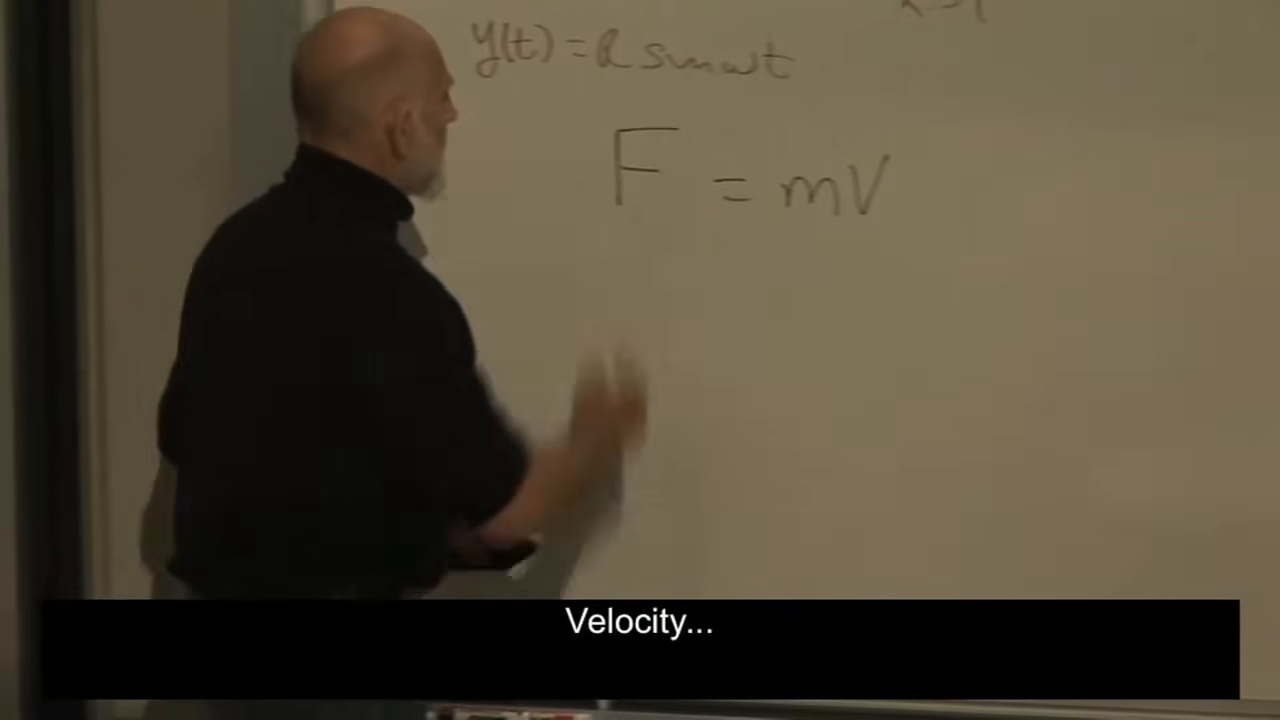
\includegraphics[width=0.82\textwidth]{lecture_02_figure_02.png}
  \caption{用來檢驗可預測性與可逆性的錯誤力--速度定律。}
  \lectureframe{00:04:51}
\end{figure}

將運動限制在一個空間座標上。由於 \(v=\dot x\)，這條定律可寫成

\begin{equation}
  F(t)=m\dot x(t).
  \label{eq:aristotle-1d}
\end{equation}

現在將時間分成長度為 \(\delta\) 的短區間。在一個區間內，

\begin{equation}
  \dot x(t)\simeq
  \frac{x(t+\delta)-x(t)}{\delta}.
  \label{eq:first-difference}
\end{equation}

將結果代入式~\eqref{eq:aristotle-1d}，得到

\begin{equation}
  x(t+\delta)
  =x(t)+\frac{\delta}{m}F(t).
  \label{eq:aristotle-update}
\end{equation}

這看起來像一條真正的更新規則：只要知道目前的位置和力，就能得出下一個頻閃時刻的位置。然而，當力為零時，亞里斯多德的規則給出 \(\dot x=0\)：物體必須維持靜止。從一開始，沒有持續施力就能保持運動的可能性便被排除在外。

\begin{figure}[htbp]
  \centering
  \includegraphics[width=0.84\textwidth]{lecture_02_figure_07.png}
  \caption{帶有恢復力的離散亞里斯多德更新。每一步都會將位移乘以略小於一的因子。}
  \lectureframe{00:10:15}
\end{figure}

\subsection{亞里斯多德力學中的彈簧}

考慮一個連接在彈簧上的粒子，其平衡位置為 \(x=0\)。粒子位移時，會受到恢復力

\begin{equation}
  F(x)=-kx,
  \qquad k>0.
  \label{eq:hooke-law}
\end{equation}

將這個力代入式~\eqref{eq:aristotle-update}，得到

\begin{equation}
  x(t+\delta)
  =\left(1-\frac{k\delta}{m}\right)x(t).
  \label{eq:aristotle-spring-update}
\end{equation}

當 \(\delta\) 足夠小時，括號中的因子略小於一。因此，每次更新都會以相同比例縮小位移：

\begin{equation}
  x_n=\left(1-\frac{k\delta}{m}\right)^n x_0.
  \label{eq:aristotle-geometric-decay}
\end{equation}

相應的連續方程及其解為

\begin{align}
  m\dot x&=-kx,
  \label{eq:aristotle-spring-continuous}\\
  x(t)&=x(0)e^{-kt/m}.
  \label{eq:aristotle-spring-solution}
\end{align}

彈簧不會振盪。粒子從任意位移處釋放後，都會以指數方式趨近原點，且越接近原點，移動得越慢。

\begin{figure}[htbp]
  \centering
  \includegraphics[width=0.84\textwidth]{lecture_02_figure_08.png}
  \caption{亞里斯多德彈簧方程的指數解。位移會衰減，而非振盪。}
  \lectureframe{00:12:02}
\end{figure}

未來很容易預測：無論初始位移為何，粒子都會趨近同一個靜止狀態。過去則是另一回事。假設我們只能以有限精度觀測到原點附近的粒子。它可能從許多不同的位移開始，因為這些位移留下的指數衰減殘量，最終都會小到落在同一個測量誤差範圍內。若有完美的數學精度，式~\eqref{eq:aristotle-spring-solution}可以反向求解；但在實際情況中，不同歷史之間的差異會逐漸被抹除。因此，從可逆的基礎動力學來看，這條定律令人起疑。

這不表示亞里斯多德的想法不合理。他描述的摩擦主導運動確實具有耗散性。問題在於，他把這種有效的描述提升為基本定律。摩擦本身也是一種力，來自複雜的微觀交互作用。手以大致固定的速度推動物體時，施力是在抵銷摩擦；施力本身並不是在產生速度。

\section{牛頓定律及其物理意義}

牛頓定律的修正之處在於：力會改變運動狀態：

\begin{equation}
  \mathbf F=m\mathbf a=m\ddot{\mathbf x}.
  \label{eq:newton-second-law}
\end{equation}

在將這條定律視為演化方程之前，必須先釐清兩個表面上的循環論證。第一個涉及參考系。人們常聽到，牛頓定律在慣性參考系中成立，而慣性參考系就是牛頓定律成立的參考系。但物理上的主張並不是這種循環定義，而是經驗性的：確實\emph{存在}某些參考系，可用適當的尺與鐘來描述，在這些參考系中，牛頓定律具有簡單的形式。相對於這些參考系加速或旋轉的參考系，則需要加入額外的表觀力。至於方程在其他參考系中如何變換，可以留待稍後推導。

第二個循環論證涉及力與質量。若把力定義為質量乘以加速度，又把質量定義為力除以加速度，這條方程看來就毫無內容。操作性實驗可以將定義與定律區分開來。先用天平讓物體與一公斤標準砝碼平衡，再在沒有其他力作用的空間中，將物體掛上彈簧秤。把彈簧固定的一小段伸長量定義為一單位的力。兩根相同的彈簧各自伸長相同的量，便提供兩單位的力，並產生兩倍的加速度。使用第二根彈簧比把一根彈簧拉長兩倍安全，因為真實的彈簧最後會進入非線性區域，甚至斷裂。若維持一根彈簧，改為連接兩個相同的質量，加速度就會減半；連接三個相同的質量，加速度則會變成三分之一。

\begin{figure}[htbp]
  \centering
  \includegraphics[width=0.84\textwidth]{lecture_02_figure_09.png}
  \caption{用來定義等量力單位並檢驗加速度與力成正比的彈簧秤思想實驗。}
  \lectureframe{00:22:45}
\end{figure}

這些比較讓下式具有經驗上的內容：

\begin{equation}
  a\propto F,
  \qquad
  a\propto\frac{1}{m},
  \qquad
  F=ma.
  \label{eq:force-mass-scaling}
\end{equation}

\emph{粒子}一詞在此泛指任何內部結構不重要的小物體，不限於基本粒子。

\subsection{為什麼單靠位置不足以描述狀態}

現在以同樣的頻閃方法檢驗牛頓方程。加速度的中心有限差分為

\begin{equation}
  \ddot x(t)\simeq
  \frac{x(t+\delta)-2x(t)+x(t-\delta)}{\delta^2}.
  \label{eq:second-difference}
\end{equation}

因此，牛頓方程意味著

\begin{equation}
  x(t+\delta)
  =2x(t)-x(t-\delta)+\frac{\delta^2}{m}F(t).
  \label{eq:newton-position-update}
\end{equation}

僅憑 \(x(t)\) 無法得出下一個位置。我們還需要前一個位置 \(x(t-\delta)\)，或等價地，需要目前時刻的速度。乍看之下，牛頓方程似乎不如亞里斯多德的方程具有預測性。正確的結論其實是：單靠位置不足以完整描述狀態。在某個時刻掌握所有相關資訊，意指掌握足以決定後續運動的資料。對牛頓力學中的粒子而言，這些資料就是位置與速度。

\section{動量與相空間}

定義動量如下：

\begin{equation}
  \mathbf p=m\mathbf v=m\dot{\mathbf x}.
  \label{eq:momentum-definition}
\end{equation}

對於固定的牛頓力學系統，質量視為常數。物體可能失去一部分，例如筆帽從筆上脫落；但此時描述的物體已經改變，而所選定的封閉系統仍有固定的總質量。當 \(m\) 保持不變時，牛頓第二定律可寫成

\begin{equation}
  \mathbf F=\dot{\mathbf p}.
  \label{eq:newton-momentum-form}
\end{equation}

\begin{figure}[htbp]
  \centering
  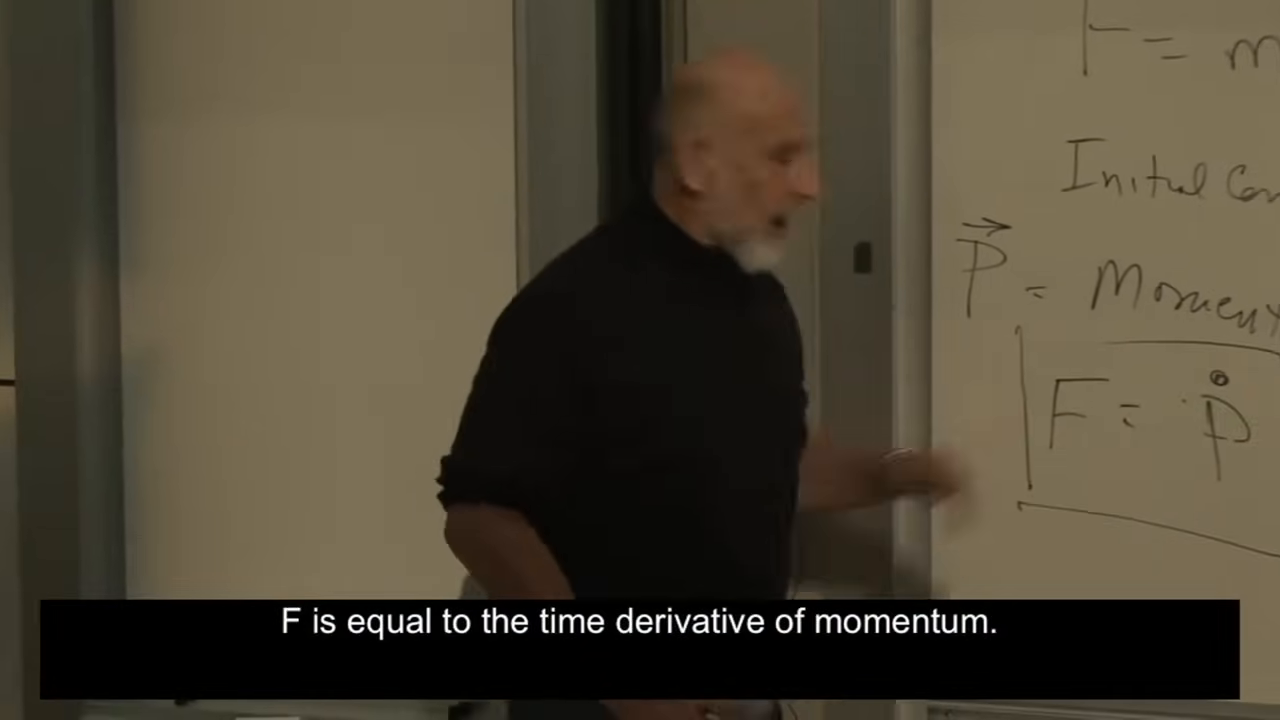
\includegraphics[width=0.82\textwidth]{lecture_02_figure_03.png}
  \caption{以動量對時間的導數表示的牛頓定律。}
  \lectureframe{00:32:35}
\end{figure}

對於一維運動，牛頓力學可寫成兩個關於兩個獨立狀態變數的一階方程：

\begin{align}
  \dot p&=F(x,t),
  \label{eq:first-order-p}\\
  \dot x&=\frac{p}{m}.
  \label{eq:first-order-x}
\end{align}

一個方程描述力如何改變動量；另一個描述動量如何改變位置。相應的一階離散形式為

\begin{align}
  p(t+\delta)&=p(t)+\delta F(x(t),t)+O(\delta^2),
  \label{eq:momentum-discrete}\\
  x(t+\delta)&=x(t)+\frac{\delta}{m}p(t)+O(\delta^2).
  \label{eq:position-discrete}
\end{align}

給定 \(x(t)\) 和 \(p(t)\) 後，這些方程便能決定下一組位置與動量；再將這組數值作為下一步的輸入。軌跡就是透過反覆更新建立起來的。

\begin{figure}[htbp]
  \centering
  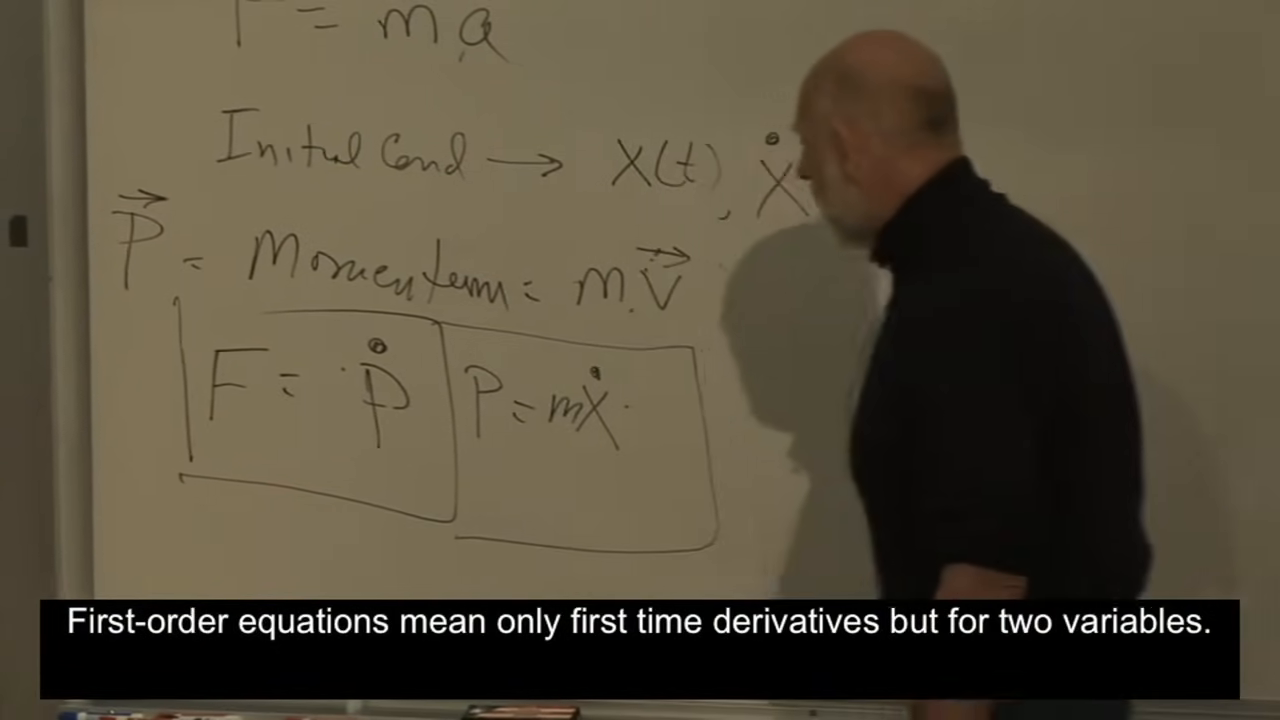
\includegraphics[width=0.84\textwidth]{lecture_02_figure_04.png}
  \caption{兩個一階方程及相應的初始資料。位置與動量合在一起指定系統的狀態。}
  \lectureframe{00:35:47}
\end{figure}

所有位置與動量配對 \((x,p)\) 所構成的空間稱為\emph{相空間}。對於在三維空間中運動的單一粒子，相空間有六個座標：

\begin{equation}
  (x,y,z,p_x,p_y,p_z).
  \label{eq:one-particle-phase-space}
\end{equation}

相空間是完整初始條件所構成的空間。位形空間只記錄位置；相空間則完整記錄運動定律所需的資料。

\begin{classroomqa}
  \audiencequestion{如果力是位置的函數，而不是已知的時間函數，更新過程會變得更複雜嗎？\lecturetimestamp{00:36:27--00:37:07}}
  \lecturerresponse{方程仍然具有預測性。一旦知道 \(x\) 和 \(p\)，就能得知 \(F(x)\) 的值。式~\eqref{eq:first-order-p}可推進 \(p\)，式~\eqref{eq:first-order-x}可推進 \(x\)，然後再次使用更新後的位置與動量。}
\end{classroomqa}

\section{牛頓力學中的彈簧}

回到彈簧問題，讓我們在相同的物理條件下比較這兩條定律。牛頓定律給出

\begin{equation}
  m\ddot x=-kx.
  \label{eq:newton-spring}
\end{equation}

暫時令 \(m=k=1\)，以消去常數。於是

\begin{equation}
  \ddot x=-x.
  \label{eq:normalized-oscillator}
\end{equation}

與指數函數不同，正弦或餘弦函數經過兩次微分後會變成自身的相反數。通解可以寫成

\begin{align}
  x(t)&=C\cos(t-t_0),
  \label{eq:oscillator-x}\\
  p(t)=\dot x(t)&=-C\sin(t-t_0).
  \label{eq:oscillator-p}
\end{align}

這兩個常數分別承載兩項初始資訊。振幅 \(C\) 給出最大位移，而 \(t_0\) 決定相位；這裡選擇相位，使粒子在 \(t=t_0\) 時速度為零。粒子只會在端點處短暫停止，接著便折返，經過原點時速率與動量最大，並繼續振盪。

將式~\eqref{eq:oscillator-x}和\eqref{eq:oscillator-p}平方，得到

\begin{equation}
  x^2+p^2=C^2.
  \label{eq:oscillator-phase-circle}
\end{equation}

因此，相空間中的點會沿半徑為 \(C\) 的圓移動。不同的初始振幅會對應到不同的圓；改變 \(t_0\)，則會在同一個圓上選擇不同的起點。在這些歸一化單位下，不論振幅為何，沿每個圓完成一周所需的週期都相同，為 \(2\pi\)。

\begin{figure}[htbp]
  \centering
  \includegraphics[width=0.84\textwidth]{lecture_02_figure_10.png}
  \caption{振子解及其在 \((x,p)\) 相平面中的圓形軌道。}
  \lectureframe{00:43:20}
\end{figure}

\begin{figure}[htbp]
  \centering
  \begin{tikzpicture}[scale=1.05,>=Latex]
    \draw[->] (-2.6,0) -- (2.75,0) node[right] {$x$};
    \draw[->] (0,-2.4) -- (0,2.55) node[above] {$p$};
    \draw[blue!65!black,thick] (0,0) circle (1.85);
    \draw[->,blue!65!black,thick]
      (1.60,0.93) arc[start angle=30,end angle=72,radius=1.85];
    \fill[red!65!black] (1.60,0.93) circle (2pt);
    \draw[dashed] (0,0) -- (1.60,0.93)
      node[midway,below right] {$C$};
    \node[align=left] at (-1.55,1.85)
      {$x=C\cos(t-t_0)$\\$p=-C\sin(t-t_0)$};
  \end{tikzpicture}
  \caption{相空間軌道同時保留位置與動量。半徑標示運動的振幅，而角度則隨時間均勻增加。}
  \label{fig:oscillator-phase-space}
\end{figure}

投影到水平軸上，得到 \(x\) 熟悉的往復運動；投影到垂直軸上，則得到 \(p\) 的振盪。亞里斯多德力學中的彈簧則不同：不同的圓不會彼此塌縮。知道相空間中的一點，就能決定系統的未來與過去。

對於一般的 \(m\) 與 \(k\)，角頻率為

\begin{equation}
  \omega=\sqrt{\frac{k}{m}},
  \qquad
  x(t)=C\cos\bigl(\omega(t-t_0)\bigr),
  \label{eq:general-oscillator-frequency}
\end{equation}

在未經縮放的 \((x,p)\) 平面中，相空間軌道會成為橢圓。講課中採用的 \(m=k=1\) 歸一化，則能方便地呈現圓形軌道。

\begin{classroomqa}
  \audiencequestion{如果把振子方程中的二階導數換成一階導數，是否就會失去可預測性？\lecturetimestamp{00:45:23--00:46:04}}
  \lecturerresponse{不會。給定適當的初始資料，一階方程仍可預測未來的運動。更深一層的問題是，方程所描述的流是否能充分保留不同狀態之間的差異，以維持可逆性。相關的一般定理，會等到具備所需的數學工具後再討論。}
\end{classroomqa}

\section{時間反演}

振子的圖像讓可逆性變得具體，但我們也可以直接檢驗方程。引入反向的時間座標

\begin{equation}
  T=-t.
  \label{eq:reverse-time}
\end{equation}

於是

\begin{equation}
  \frac{d}{dt}=-\frac{d}{dT},
  \qquad
  \frac{d^2}{dt^2}=\frac{d^2}{dT^2}.
  \label{eq:time-derivative-parity}
\end{equation}

時間反演會使一階導數變號，但不會改變二階導數。因此，自治的亞里斯多德方程

\begin{equation}
  m\dot x=F(x)
  \label{eq:aristotle-time-reversal}
\end{equation}

在影片倒放時不再具有相同形式。衰減的彈簧倒放後，會變成自行離開平衡位置的彈簧。相較之下，

\begin{equation}
  m\ddot x=F(x)
  \label{eq:newton-time-reversal}
\end{equation}

則維持原有形式。牛頓運動的影片倒放時，速度會反向，但加速度保持不變，因此倒放後的運動仍是方程允許的解。

\begin{figure}[htbp]
  \centering
  \includegraphics[width=0.84\textwidth]{lecture_02_figure_11.png}
  \caption{在 \(t\mapsto -t\) 變換下比較板書：一階導數變號，二階導數則不變。}
  \lectureframe{00:50:45}
\end{figure}

\begin{classroomqa}
  \audiencequestion{為什麼應將可逆性視為一般物理定律的前提？\lecturetimestamp{00:46:16--00:48:26}}
  \lecturerresponse{可逆性是經由檢驗而接受的，不是由定義保證的。我們考察成功的定律，找出它們共同的實驗特徵，再將這些特徵提升為原理。更深層的邏輯順序其實相反：量子場論更為基本，而牛頓力學則透過慢速運動、重物體等近似而出現。課程必須從較簡單的定律逐步建立，因此現在先將可逆性引入為一項原理，日後再檢驗它的適用範圍。}
\end{classroomqa}

\begin{classroomqa}
  \audiencequestion{牛頓是否曾有意識地將可逆性視為一個問題？\lecturetimestamp{00:48:28--00:49:02}}
  \lecturerresponse{歷史上的答案並不確定。牛頓確實理解慣性：改變運動狀態需要力，維持等速運動則不需要力。至於他是否曾明確地從可逆性的角度表述這項洞見，則是另一個歷史問題。}
\end{classroomqa}

\section{週期運動與守恆量}

相空間中的圓帶出下一個想法。軌跡始終留在同一個圓上，不會跳到另一個圓。因此，可以用一個沿運動保持不變的數值來標記這個圓。對於歸一化振子，這個數值是

\begin{equation}
  C^2=x^2+p^2.
  \label{eq:cycle-label}
\end{equation}

這就是振子的能量，相差一個二分之一的因子。半徑較大的圓具有較大的能量；改變起始相位並不會改變能量。我們會推導這個結論，而不是只從圖像中讀出來；不過，先來考慮動量。

牛頓第一定律指出，若物體所受合力為零，它就會以固定速度運動。這項定律已包含在第二定律中：

\begin{equation}
  \mathbf F=0
  \quad\Longrightarrow\quad
  \dot{\mathbf p}=0
  \quad\Longrightarrow\quad
  \mathbf v=\text{constant}
  \label{eq:newton-first-from-second}
\end{equation}

其中質量為常數。牛頓第三定律則提供了關於粒子間交互作用的真正新資訊。

\subsection{大小相等、方向相反且沿連心線的力}

令 \(\mathbf F_{ij}\) 表示粒子 \(i\) 受到粒子 \(j\) 施加的力。牛頓第三定律中大小相等、方向相反的部分是

\begin{equation}
  \mathbf F_{ij}=-\mathbf F_{ji}.
  \label{eq:newton-third-pair}
\end{equation}

如果這兩個力指向相同方向，一對孤立粒子就可能自發加速。這就成了不需要推進劑、只靠內力產生運動的機器；我們並未觀察到這種情形。

\begin{figure}[htbp]
  \centering
  \includegraphics[width=0.84\textwidth]{lecture_02_figure_12.png}
  \caption{以指標表示的交互作用力大小相等、方向相反關係。}
  \lectureframe{00:59:25}
\end{figure}

對於此處討論的點粒子力，這對作用力還沿著連接兩粒子中心的直線。如果大小相等、方向相反的力不在同一直線上，就可能形成純力矩，使一對孤立的剛體開始旋轉。沿連心線作用的條件排除了這種可能性：

\begin{equation}
  \mathbf F_{ij}\parallel
  (\mathbf r_i-\mathbf r_j).
  \label{eq:central-force-condition}
\end{equation}

大小相等、方向相反的條件將導出線動量守恆。沿連心線作用的條件則與角動量守恆有關，之後會再討論。

\begin{figure}[htbp]
  \centering
  \includegraphics[width=0.84\textwidth]{lecture_02_figure_13.png}
  \caption{牛頓第三定律中沿連心線作用的部分：交互作用力沿著連接兩粒子的直線作用。}
  \lectureframe{01:01:38}
\end{figure}

\subsection{總動量}

考慮一個包含 \(N\) 個粒子的封閉系統。系統沒有外力，只有粒子彼此施加的力。由力的可加性與牛頓第二定律可得，對每個粒子而言：

\begin{equation}
  \dot{\mathbf p}_i
  =m_i\ddot{\mathbf r}_i
  =\sum_{\substack{j=1\\j\ne i}}^N \mathbf F_{ij}.
  \label{eq:many-particle-newton}
\end{equation}

將此方程對 \(i\) 求和：

\begin{align}
  \frac{d}{dt}\sum_{i=1}^N\mathbf p_i
  &=\sum_{i=1}^N
    \sum_{\substack{j=1\\j\ne i}}^N\mathbf F_{ij}
  \notag\\
  &=\sum_{i<j}\bigl(\mathbf F_{ij}+\mathbf F_{ji}\bigr)
  =0.
  \label{eq:momentum-pair-cancellation}
\end{align}

每一組交互作用力都會出現兩次，分別代表作用力與反作用力，兩者相互抵銷。定義

\begin{equation}
  \mathbf P_{\mathrm{tot}}=\sum_{i=1}^N\mathbf p_i,
  \label{eq:total-momentum}
\end{equation}

便得到第一個守恆定律：

\begin{equation}
  \frac{d\mathbf P_{\mathrm{tot}}}{dt}=0.
  \label{eq:momentum-conservation}
\end{equation}

\begin{figure}[htbp]
  \centering
  \includegraphics[width=0.84\textwidth]{lecture_02_figure_14.png}
  \caption{將各粒子的方程相加後，成對的作用力會相互抵銷，留下總動量的時間導數為零。}
  \lectureframe{01:04:38}
\end{figure}

從歷史發展的角度來看，我們將動量守恆視為牛頓第三定律的推論。現代物理學往往把動量守恆看得更基本：如果一個孤立的雙粒子系統總動量守恆，內部動量的變化就必須大小相等、方向相反。不過，在目前的推導脈絡中，採用牛頓力學的推導方式較為合適。

\section{一維能量}

考慮一個粒子在直線上運動，所受的力只取決於位置：

\begin{equation}
  F=F(x).
  \label{eq:position-force}
\end{equation}

這種力稱為不顯含時間的力。這不表示運動中的粒子所受之力數值固定；力的數值會隨著 \(x(t)\) 改變。它的意思是，無論鐘錶顯示的時間為何，只要粒子位於相同位置 \(x\)，所受的力就相同。

在一維中，任何足夠平滑的力函數都可以積分。因此我們定義勢能 \(V(x)\) 如下：

\begin{equation}
  F(x)=-\frac{dV}{dx},
  \label{eq:potential-definition-1d}
\end{equation}

或等價地寫成

\begin{equation}
  V(x)=-\int^x F(u)\,du+V_0.
  \label{eq:potential-integral}
\end{equation}

加法常數 \(V_0\) 不會影響力。可以把 \(V(x)\) 想成 \(x\) 軸上方地形的高度。粒子會受到指向較低處的力，斜率越陡，力越大。在平滑山丘的頂端或底部，斜率為零，因此力也為零。

\begin{figure}[htbp]
  \centering
  \includegraphics[width=0.84\textwidth]{lecture_02_figure_15.png}
  \caption{以一維地形表示勢能。力指向下坡方向，大小由斜率決定。}
  \lectureframe{01:12:57}
\end{figure}

定義動能、勢能與總能量如下：

\begin{equation}
  T=\frac12m\dot x^2,
  \qquad
  E=T+V(x)
  =\frac12m\dot x^2+V(x).
  \label{eq:energy-1d}
\end{equation}

此時，能量只是我們給這個可能守恆的量取的名稱。地形圖提供了它的物理解釋：粒子往下移動時，\(V\) 會降低，速度則會增加，因此 \(T\) 也會增加；往上移動時則相反。牛頓方程可以證明，這兩者之間的轉換恰好相等。

對式~\eqref{eq:energy-1d}微分。由於 \(m\) 是常數，而 \(V\) 只透過 \(x(t)\) 隨時間改變，

\begin{align}
  \frac{dE}{dt}
  &=m\dot x\ddot x+\frac{dV}{dx}\dot x
  \notag\\
  &=\dot x\left(m\ddot x+\frac{dV}{dx}\right).
  \label{eq:energy-derivative-1d}
\end{align}

根據牛頓定律與 \(V\) 的定義，

\begin{equation}
  m\ddot x=F=-\frac{dV}{dx}.
  \label{eq:newton-potential-1d}
\end{equation}

因此，式~\eqref{eq:energy-derivative-1d}中的括號項為零：

\begin{equation}
  \frac{dE}{dt}=0.
  \label{eq:energy-conservation-1d}
\end{equation}

\begin{figure}[htbp]
  \centering
  \includegraphics[width=0.84\textwidth]{lecture_02_figure_16.png}
  \caption{一維能量的時間導數可寫成速度乘以牛頓方程。}
  \lectureframe{01:19:18}
\end{figure}

在一維中，只要力是足夠平滑且依賴位置，就不需要其他動力學假設，因為這類力都存在原函數。

\section{多維情形與保守力}

對於座標為 \(x_i\) 的粒子，牛頓方程的各分量為

\begin{equation}
  F_i(\mathbf x)=m\ddot x_i.
  \label{eq:newton-components}
\end{equation}

力的分量 \(F_i\) 可能取決於所有座標，而不只取決於 \(x_i\)。我們希望找到一個純量函數 \(V(\mathbf x)\)，使得

\begin{equation}
  F_i(\mathbf x)
  =-\frac{\partial V(\mathbf x)}{\partial x_i},
  \qquad
  \mathbf F=-\boldsymbol\nabla V.
  \label{eq:gradient-force}
\end{equation}

這不像一維的構造那樣必然成立。三個任意函數 \(F_1,F_2,F_3\) 通常包含比單一純量函數的各偏導數更多的獨立資訊。換句話說，只有在力場滿足相容條件時，才存在勢能；例如，相應的混合偏導數必須相等。在單連通區域中，這個條件可寫為 \(\boldsymbol\nabla\times\mathbf F=0\)。
因此，我們將式~\eqref{eq:gradient-force}視為適用於此處所討論力類別的物理假設，而非數學恆等式。

\begin{figure}[htbp]
  \centering
  \includegraphics[width=0.84\textwidth]{lecture_02_figure_17.png}
  \caption{多維力定律與勢能等高線示意圖。力穿過等高線，指向 \(V\) 減小的方向。}
  \lectureframe{01:24:15}
\end{figure}

在等高線圖上，\(V\)沿著每條等高線保持不變。梯度垂直於等高線，並指向上升最快的方向；力 \(-\boldsymbol\nabla V\) 則指向下降最快的方向。

\begin{figure}[htbp]
  \centering
  \begin{tikzpicture}[scale=1.0,>=Latex]
    \draw[->] (-3.0,0) -- (3.1,0) node[right] {$x_1$};
    \draw[->] (0,-2.4) -- (0,2.55) node[above] {$x_2$};
    \draw[orange!65!black,thick]
      plot[smooth cycle] coordinates
      {(-0.55,-0.35) (0.15,-0.55) (0.72,-0.10) (0.50,0.53) (-0.25,0.65)};
    \draw[orange!65!black,thick]
      plot[smooth cycle] coordinates
      {(-1.15,-0.75) (0.20,-1.10) (1.35,-0.25) (1.10,0.95) (-0.45,1.25)};
    \draw[orange!65!black,thick]
      plot[smooth cycle] coordinates
      {(-1.85,-1.20) (0.15,-1.70) (2.15,-0.40) (1.70,1.50) (-0.80,1.85)};
    \draw[->,blue!65!black,very thick] (1.62,0.73) -- (0.82,0.20)
      node[midway,above left] {$\mathbf F$};
    \draw[dashed,->,red!65!black,thick] (0.82,0.20) -- (1.62,0.73)
      node[midway,below right] {$\boldsymbol\nabla V$};
    \node[orange!65!black] at (-1.62,1.45) {$V=V_3$};
    \node[orange!65!black] at (-0.92,0.92) {$V=V_2$};
    \node[orange!65!black] at (-0.35,0.30) {$V=V_1$};
  \end{tikzpicture}
  \caption{純量勢的等高線。梯度垂直於等高線；保守力則指向相反方向。}
  \label{fig:potential-contours}
\end{figure}

若式~\eqref{eq:gradient-force}成立，定義

\begin{equation}
  E=\frac12m\sum_i\dot x_i^2+V(x_1,\ldots,x_n).
  \label{eq:energy-many-coordinates}
\end{equation}

動能項等於質量的一半乘以速度向量長度的平方。對其微分並使用多變數鏈鎖律，得到

\begin{align}
  \frac{dE}{dt}
  &=m\sum_i\dot x_i\ddot x_i
    +\sum_i\frac{\partial V}{\partial x_i}\dot x_i
  \notag\\
  &=\sum_i\dot x_i
    \left(m\ddot x_i+\frac{\partial V}{\partial x_i}\right)
  =0.
  \label{eq:energy-derivative-multidimensional}
\end{align}

這項證明與一維情形完全相同，只是多了指標；但前提更強：所有力分量都必須源自同一個勢能。

\begin{figure}[htbp]
  \centering
  \includegraphics[width=0.84\textwidth]{lecture_02_figure_18.png}
  \caption{帶有指標的能量導數。每個括號項都根據牛頓方程的相應分量而為零。}
  \lectureframe{01:28:30}
\end{figure}

對於三維空間中的 \(N\) 個粒子，將所有座標依序列出

\begin{equation}
  \begin{aligned}
    q_a={}&(x_1,y_1,z_1,x_2,y_2,z_2,\ldots,\\[-0.2em]
           &\phantom{(}x_N,y_N,z_N),\\
    &a=1,\ldots,3N.
  \end{aligned}
  \label{eq:flattened-coordinates}
\end{equation}

共有 \(3N\) 個座標分量，但只有 \(N\) 個粒子的質量；每個粒子的三個座標分量都使用同一個質量。若

\begin{equation}
  F_a=-\frac{\partial V(q_1,\ldots,q_{3N})}{\partial q_a},
  \label{eq:many-particle-conservative-force}
\end{equation}

則

\begin{equation}
  E=\sum_{A=1}^{N}\frac12m_A\lvert\dot{\mathbf r}_A\rvert^2
    +V(\mathbf r_1,\ldots,\mathbf r_N)
  \label{eq:many-particle-energy}
\end{equation}

根據相同的推導，這個量守恆。由勢能導出的力稱為\emph{保守}力，正是因為它們使這項守恆定律成立；這裡的「保守」一詞與政治立場無關。

\section{以能量等高線呈現的振子}
\enlargethispage{3\baselineskip}

對於彈簧力 \(F=-kx\)，由式~\eqref{eq:potential-definition-1d}可得

\begin{equation}
  V(x)=\frac12kx^2+V_0.
  \label{eq:spring-potential}
\end{equation}

選擇 \(V_0=0\) 後，振子的能量為

\begin{equation}
  E=\frac12m\dot x^2+\frac12kx^2
   =\frac{p^2}{2m}+\frac12kx^2.
  \label{eq:oscillator-energy}
\end{equation}

當 \(m=k=1\) 時，

\begin{equation}
  2E=p^2+x^2=C^2.
  \label{eq:oscillator-energy-circle}
\end{equation}

因此，先前得到的相空間圓就是等能線。對於更一般的一維勢能，等能線不一定是圓，但運動仍會沿著曲線進行：

\begin{equation}
  \frac{p^2}{2m}+V(x)=E
  \label{eq:general-energy-contour}
\end{equation}

曲線位於 \((x,p)\) 平面中。這讓我們回到第一講的想法：當軌跡始終留在彼此不同的週期軌道上時，可以用一個數值標記這些軌道，而且該數值在運動過程中保持不變。

現在我們已經有了狀態空間、牛頓力學的更新方程，以及前兩項守恆定律。接下來將介紹力學的另一種表述，從最小作用量原理出發，導向拉格朗日量、哈密頓量、角動量，以及這些例子背後更一般的結構。

\begin{classroomqa}
  \audiencequestion{發下來的講義和黑板上的內容有多一致？圖在哪裡？\lecturetimestamp{01:37:56--01:38:54}}
  \lecturerresponse{講義應該會緊跟課堂內容；如果黑板上的內容沒有收錄，可能是寄錯了檔案。圖還沒準備好；他開玩笑說，等繼續教育部門支付下一張支票時，圖就會出現。}
\end{classroomqa}